{
% Zähler „fibelbeerctr“ und „fibeltotalbeerscore“ werden für den
% \fibelbeertable-Befehl gebraucht
\newcounter{fibelbeerctr}
\newcounter{fibeltotalbeerscore}

% Befehl \fibelbeerscore: Wandelt die angegebene Zahl in eine entsprechende
% 	Anzahl von Bildern („Bierpunkten“) um
\newcommand{\fibelbeerscore}[1]{
	\addtocounter{fibeltotalbeerscore}{#1}
	\forloop{fibelbeerctr}{0}{\value{fibelbeerctr} < #1}{%
		\raisebox{-1mm}{
\includegraphics[width=5mm]{res/beerpoint.pdf}}%
		\hspace{0.6em}%
	}%
	\hspace{-0.6em}
}

% Die verschiedenen Kategorien für die Punktzahl-Tabelle
\makeatletter
\newcommand{\sauberkeit}{0}
\define@key{fibelbeer}{sauberkeit}{\renewcommand{\sauberkeit}{#1}}
\newcommand{\preisleistung}{0}
\define@key{fibelbeer}{preisleistung}{\renewcommand{\preisleistung}{#1}}
\newcommand{\gemuetlichkeit}{0}
\define@key{fibelbeer}{gemuetlichkeit}{\renewcommand{\gemuetlichkeit}{#1}}
\newcommand{\groesse}{0}
\define@key{fibelbeer}{groesse}{\renewcommand{\groesse}{#1}}
\newcommand{\happyhour}{0}
\define@key{fibelbeer}{happyhour}{\renewcommand{\happyhour}{#1}}
\newcommand{\flirtfaktor}{0}
\define@key{fibelbeer}{flirtfaktor}{\renewcommand{\flirtfaktor}{#1}}
\makeatother

% Befehl \fibelbeertable: Erstellt eine Tabelle mit den Bierpunkt-Bewertungen
% für eine Disco/Kneipe (inkl. berechneter Gesamtpunktzahl)
%	Parameter: Punktzahlen (0–5) werden in der Form
%	\fibelbeertable{sauberkeit=<zahl>, …} übergeben.
\newcommand{\fibelbeertable}[1]{
	\begin{minipage}{\columnwidth}
		\setkeys{fibelbeer}{#1}
		\setcounter{fibeltotalbeerscore}{0}
		\centering
		\small
		\begin{tabular}{| l | >{\raggedright\arraybackslash}m{3.45cm} |}
			\hline
			Sauberkeit		& \fibelbeerscore{\sauberkeit} \\ \hline
			Preis/Leistung	& \fibelbeerscore{\preisleistung} \\ \hline
			Gemütlichkeit	& \fibelbeerscore{\gemuetlichkeit} \\ \hline
			Happy Hour		& \fibelbeerscore{\happyhour} \\ \hline
			Flirtfaktor		& \fibelbeerscore{\flirtfaktor} \\ \hline
		\end{tabular}\\\medskip
		
		\textbf{Bierpunktzahl insgesamt: \arabic{fibeltotalbeerscore}/25}
		
		\smallskip
		\raggedright
		\hspace{0.2\columnwidth}
		Größe: \fibelbeerscore{\groesse}
	\end{minipage}
}

% „secnumdepth“ zwischenspeichern
\setcounter{fibtemp}{\value{secnumdepth}}
% Automatisch „Kneipe #: “ vor \subsection schreiben
\setcounter{secnumdepth}{\subsectionnumdepth}
\renewcommand{\subsectionformat}{Kneipe \arabic{subsection}: }
% Abstände bei \subsection reduzieren (wie bei \subsubsection)
\fibelspacingsubsubsection[subsection]

\section{Der Kneipen-Guide!}
\begin{multicols*}{2}
\textbf{Was darf man neben dem Studium auf keinen Fall vergessen?
	Na, wer weiß es?\\
	Richtig, einen gemütlichen Kneipenabend.
	Damit ihr wisst, wo das in Münster am besten geht, stellen wir euch hier den ultimativen Kneipenguide vor.}

Da wir Kneipen bewerten, werden wir ganz stilecht Bierpunkte in den einzelnen Kategorien vergeben.
In jeder dieser Kategorien können maximal fünf Bierpunkte erreicht werden.
Hier unsere folgenden fünf Bewertungskategorien:
\begin{description}
	\item[Sauberkeit:] Hier testen wir die Sauberkeit, die Hygiene der Toiletten sowie die Sauberkeit im Thekenbereich und der gesamten Räumlichkeit.
	\item[Preis/Leistung:] Hier testen wir, wie zum Beispiel die Getränkegröße im Verhältnis zum Preis steht, und was man für sein bezahltes Eintrittsgeld geboten bekommt.
	\item[Gemütlichkeit:] Hier testen wir z.\,B.\ die Sitzmöglichkeiten und die Lautstärke der Musik.
	\item[Happy Hour:] Hier testen wir den zeitlichen Umfang und zudem das Angebot der Happy Hour.
	\item[Flirtfaktor:] Hier bewerten wir, wie die Singlequote sowie das Flirtverhalten der Partypeople in den jeweiligen Locations ist.
	Unsere Bewertung bezieht sich auf Erfahrungsberichte diverser Testpersonen ;-)
\end{description}

\begin{center}
	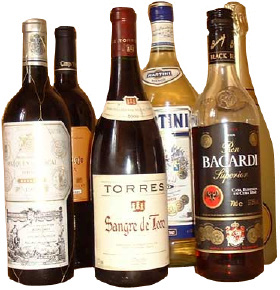
\includegraphics[width=\columnwidth, height=0.22\textheight]{res/kneipenguide_flaschen.png}
\end{center}

Außerdem geben wir für jedes Lokal die Größe der Räumlichkeiten an, damit ihr euch darauf einstellen könnt, ob das Feeling eher Sardellendose oder Stadion (oder am besten irgendwo dazwischen) ist.

\subsection{Cavete}
Die Cavete ist wohl die unter Studenten weit verbreitetste Kneipe, und dies hat ihre Gründe: Zum Einen ist die Kneipe ursprünglich von Studenten für Studenten errichtet worden.
Entsprechend gut gefüllt ist die Kneipe an freien Tagen, beziehungsweise in den Nächten vor diesen.
Von ihren Betreibern wird die Cavete als "urig eingerichtet" beschrieben, und dem ist nichts entgegenzusetzen:
Bereits wenn man den ersten Schritt über die Schwelle tut, blickt man auf eine verzierte Holzwand.
Ob die Verzierung schön ist, liegt im Auge des Betrachters.
Tische, Stühle und der größte Teil der Innenarchitektur sind tatsächlich hölzern -- oder wirken zumindest so.

Erwähnenswert ist, dass es jeden Tag bis 23~Uhr eine warme Küche gibt.
Verspeisen könnt ihr hier Pommes, Currywurst und auch Nachos.
Aber auch "große" Gerichte wie Lachs, Schnitzel oder Nudeln.
Die Auswahl der Getränke lässt auch keineswegs zu wünschen übrig und ihr könnt zwischen Softdrinks, Bier, Longdrinks, Schnaps und Cocktails auswählen.
Selbstverständlich fehlt auch die typische "Happy Hour" nicht, in welcher ihr ab 20~Uhr jeden Cocktail um \num{1,40}~Euro günstiger bekommt.
Die Atmosphäre ist meist -- und das heißt immer dann, wenn die Kneipe nicht hoffnungslos überfüllt ist -- sehr angenehm, man kann sich mühelos unterhalten, Karten spielen und hat de facto keine Probleme mit anderen Kneipenbesuchern aka "Stress".

Die Kneipe hat jeden Abend ab 18~Uhr geöffnet und sollte von jedem Studenten
einmal besucht worden sein.

\begin{center}
	\fibelbeertable{sauberkeit=2, preisleistung=4, gemuetlichkeit=5, groesse=3, happyhour=3, flirtfaktor=4}
\end{center}

\subsection{Enchilada}
Das Enchilada ist eine mexikanische Bar, welche besonders für ihr reichhaltiges Angebot an wohlschmeckenden Cocktails bekannt ist.
Ein Besuch empfiehlt sich montags, dann ist nämlich "Casino-Tag":
Man geht zum Barkeeper, bestellt einen Cocktail, würfelt und bezahlt die Augenzahl.
Empfehlenswert also für alle, die beim "Mensch ärgere dich nicht" immer verlieren.
Zudem gibt es mexikanisches Essen, unter anderem -- natürlich -- Enchiladas.
Die Happy Hour geht bis 20~Uhr, die "Enchilada Hour" beginnt ab 23~Uhr.
Das Restaurant liegt etwas versteckt in der Arztkarrengasse~12 in Bahnhofs- und Innenstadtnähe.

\begin{center}
	\fibelbeertable{sauberkeit=4, preisleistung=4, gemuetlichkeit=3, groesse=4, happyhour=5, flirtfaktor=4}
\end{center}

\subsection{Destille}
Viele Worte muss man zur "Dille", wie sie eigentlich immer nur genannt wird, eigentlich nicht verlieren.
Jeder Münsteraner kennt diese Kneipe, die im absoluten Kneipenzentrum Münsters in der Jüdefelderstraße gelegen ist.
Die Destille selbst ist an der Ecke zur Kuhstraße (Hausnummer~10 auf dieser).
Trotz der Kneipenflut dort hat sie es irgendwie geschafft, nicht unterzugehen und für jeden in Münster ein Begriff zu sein.

Die Dille ist ein gutes Ziel, wenn man sich vollaufen lassen will.
Die Preise sind relativ günstig und für das Kneipenviertel damit durchaus konkurrenzfähig.
Ein dementsprechendes Klientel ist dort auch anzutreffen -- aber in der Jüdefelderstraße sollte man das ohnehin erwarten.
Man kann auch nicht sagen, dass in der Dille viel Wert auf Sauberkeit, Deko oder Stil gelegt wird.
Wenn ihr ausgiebig und laut feiern wollt, ist das ja aber vielleicht genau das Richtige für euch.

Die Happy Hour ist hier um 20:00--21:30~Uhr, u.\,a.\ mit Long Island für günstige \SI{4}{\euro}.

\begin{center}
	\fibelbeertable{sauberkeit=1, preisleistung=4, gemuetlichkeit=2, happyhour=5, flirtfaktor=2, groesse=3}
\end{center}

\subsection{Kruse Baimken}
Beim "krausen Bäumchen" handelt es sich um einen traditionsreichen, bayrisch angehauchten Biergarten, in dem sogar schon Angela Merkel zu Gast war.
Geboten wird bürgerliche Küche sowie eine gute Auswahl an Getränken.
Hervorstechendes Merkmal ist die Lage: Direkt am Aasee, weshalb ein Besuch vor allem bei schönem Wetter zu empfehlen ist.
Ein Pils (\SI{0,3}{\l}) ist für \SI{2,90}{\euro} zu haben (Stand 08/15).

\begin{center}
	\fibelbeertable{sauberkeit=5, preisleistung=3, gemuetlichkeit=5, groesse=4, happyhour=0, flirtfaktor=2}
\end{center}

\subsection{Fegefeuer}
Für alle ehrenwerten Ritter und holden Burgfräulein des Münsterlandes bietet diese mittelalterliche Kaschemme den perfekten Ort, um mit ein oder zwei schwarzen Äbten auf die nächste Schlacht anzustoßen.
Auch für Freunde der mittelalterlich-experimentellen Cuisine hat das Fegefeuer für 4--20\,€ einiges zu bieten; die meisten Henkersmähler gibts auch vegetarisch oder vegan! Die Bier- und Metpreise sind human (ca.\ \SI{2,60}{\euro} für \SI{0,3}{\l} Bier/\SI{0,1}{\l} Met), die Atmosphäre ist in Münster einzigartig und die Bedienung ist mittelalterlich gewandet.
Vorsicht! Nicht vom neckisch-ruppigen Umgangston abschrecken lassen.

\begin{center}
	\fibelbeertable{sauberkeit=5, preisleistung=5, gemuetlichkeit=5, happyhour=0, flirtfaktor=1, groesse=3}
\end{center}

\subsection{Watusi Bar} % 2018 geprüft
Die Watusi Bar ist eine Hafenkneipe und findet sich in der Dortmunder Straße~34.
Wenn man sich im Gefilde der Münsteraner Studentenkneipen nicht auskennt, wirkt das vielleicht etwas abgelegen, allerdings ist die Watusi Bar eine Studenten-Cocktail-Bar wie sie im Buche steht.
Wenn man drinnen auf einem der Sofas sitzt, kann man durchaus für einen kurzen Moment glauben, man säße in der Studenten-WG eines Kumpels und nicht in einer Bar.
Die Toilette ist klassisch mit einer übertriebenen Menge von Plakaten, Aufklebern und Edding-Kritzeleien übersät, allerdings auch leider nicht wirklich sauber.
Im warmen Sommer kann man auch sehr gut draußen auf den Bänken sitzen und den angeregten Gesprächen lauschen.

Kernangebot der Watusi Bar sind natürlich ihre Cocktails!
Das Angebot ist mit Preisen von \SIrange{4,5}{6}{\euro} überwältigend günstig, was durch eine großzügige Happy Hour sogar noch weiter getrieben wird.
Das heißt aber nicht, dass die Cocktails nicht gut schmecken.
Wer einmal solche Kreationen wie das "Kettensägenmassaker", "Schlock, das Bananenmonster" oder "Princess Peach" probieren möchte, sollte einen Besuch der Watusi Bar nicht verpassen.

Durch die Lage im Hafen ist die Nähe zu den restlichen Hafen-"Institutionen" wie dem Amp oder der Sputnikhalle (oder auch dem Kino) gegeben.
Je nachdem, zu welcher Zeit man auftaucht, kann man sehr viele oder sehr wenige Menschen in der Watusi Bar antreffen -- immerhin hat sie 19--4~Uhr geöffnet.

\begin{center}
	\fibelbeertable{sauberkeit=2, preisleistung=5, gemuetlichkeit=4, happyhour=4, flirtfaktor=3, groesse=2}
\end{center}

\subsection{Bohème Boulette}
Die liebevoll "Bulätte" genannte Kneipe liegt am Hansaring und bietet somit eine gute Alternative zu den eher teuren, nahegelegenen Hafenkneipen.
Sie ist gemütlich wie Omas Wohnzimmer und bietet Bier und Burger zu absolut menschlichen Preisen an.
Die Burger sind übrigens der absolute Oberhammer!

\begin{center}
	\fibelbeertable{sauberkeit=4, preisleistung=4, gemuetlichkeit=4, happyhour=1, flirtfaktor=2, groesse=2}
\end{center}

\subsection{Lieschen Müller} % 2018 geprüft
Das Lieschen Müller ist zentral gelegen und hat eine relativ entspannte Atmosphäre. Hier gibt es regelmäßig Quizabende, Tatort-Abende und Auftritte von "Menschen mit Gitarre". (Es eignet sich also gut, um mit kulturinteressierten Leuten einen netten Abend zu verbringen, nicht jedoch für sinnlose Besäufnisse.) Das Lieschen ist gleichzeitig Kneipe und Café, man kann also auch nachmittags zu Kaffee und Kuchen hier einkehren (Burger gibt es auch.) Erwähnenswert ist, dass man hier Tischtennis spielen kann!

Bierpreis 2,80€ für 0,33l

\begin{center}
	\fibelbeertable{sauberkeit=4, preisleistung=3, gemuetlichkeit=4, happyhour=0, flirtfaktor=4, groesse=2}
\end{center}

% secnumdepth zurücksetzen
\setcounter{secnumdepth}{\value{fibtemp}}
\subsection{Tipps \& Tricks im Nachtleben}
Hier zum Schluss noch ein paar Sachen, die wir euch mit auf den Weg geben wollen.
\begin{itemize}[labelsep=*, leftmargin=1.2em]
	\item Besucht auf jeden Fall die zahlreichen Partys für Erstsemester, die am Anfang des Semesters angeboten werden.
	\item Probiert es aus auch mal, mittwochs feiern zu gehen.
	Ist zwar am anderen Tag meist Uni, aber es lohnt sich, da sehr viele Studenten an diesem Tag unterwegs sind.
	\item Geht am besten nicht zu früh in die Klubs, ab 24~Uhr kann man sie gut ansteuern.
	In die Altstadt kann man an sich nicht zu früh gehen.
	Ab 21~Uhr ist hier am Wochenende oftmals schon was los.
	Vorher lohnt es sich vorzutrinken, denn auch wenn die Happy Hours oft gut sind, geht so ein geiler Abend schnell ins Geld.
	\item Wenn ihr im Sommer nicht unbedingt Lust habt, in einer stickigen Kneipe zu sitzen, ist es total schön, sich mit ein paar Freunden einen Kasten Bier zu kaufen, und sich gemütlich an den Aasee oder Kanal zu setzen.
	Ihr werdet feststellen, dass man im Sommer viele Studenten dort trifft, die sich zu einem gemütlichen Bierchen im Freien treffen.
\end{itemize}

\fibelsig{Michael, Raffi, Valentin, Simon, Silke, Annika}
\end{multicols*}

}
